%!TEX TS-program = lualatex
%!TEX encoding = UTF-8 Unicode

\documentclass[12pt, addpoints]{exam}

%\printanswers

\usepackage[left=1in,right=0.75in,top=1in]{geometry}     

\usepackage{fontspec}
\def\mainfont{Linux Libertine O}
\setmainfont[Ligatures=TeX, Contextuals={NoAlternate}, BoldFont={* Bold}, ItalicFont={* Italic}, Numbers={Proportional, OldStyle}]{\mainfont}
\setsansfont[Scale=MatchLowercase]{Linux Biolinum O} 
\usepackage{microtype}

\usepackage{graphicx}
	\graphicspath{%
	{/Users/goby/Pictures/teach/300/exams/}
	{/Users/goby/pictures/teach/438/exam/}}%

% Used to get the last two digits of the year for the header below.
\def\short#1{\csname @gobbletwo\expandafter\endcsname\number#1}

\pagestyle{headandfoot}
\firstpageheader{Evolution, Exam 3, Sp\short{\year}.}{}{%
	\ifprintanswers\textbf{KEY}\else Name: \enspace \makebox[2.5in]{\hrulefill}\fi}
\runningheader{}{}{\small{pg. \thepage}}

\footer{\iflastpage{\small \rule{0.6in}{0.4pt} / \numpoints\ points}{}}{}{\iflastpage{\small Have a great summer!}{}}%{\makebox[0.75in]{\hrulefill}}
\extrafootheight{-0.5in}

\pointsinmargin
\marginpointname{ pts}
\marginbonuspointname{ pts \textsc{e.c.}}

\usepackage{multicol}
\usepackage{booktabs}
\usepackage{enumitem}

%% Remove comment %% to print answer key.
\unframedsolutions
\renewcommand{\solutiontitle}{}
\SolutionEmphasis{\bfseries}

%% Create a Matching question format
\newcommand*\Matching[1]{
\ifprintanswers
	\textbf{#1}
\else
	\rule{2.1in}{0.5pt}
\fi
}

\newlength\matchlena
\newlength\matchlenb
\settowidth\matchlena{\rule{2.1in}{0pt}}
\newcommand\MatchQuestion[2]{%
	\addtocounter{numpoints}{2}
	\setlength\matchlenb{\linewidth}
	\addtolength\matchlenb{-\matchlena}
	\parbox[t]{\matchlena}{\Matching{#1}}\enspace\parbox[t]{\matchlenb}{#2}}


\newcommand*\AnswerBox[2]{%
    \parbox[t][#1]{0.92\textwidth}{%
    \begin{solution}#2\end{solution}}
    \vspace*{\stretch{1}}
}

\newenvironment{AnswerPage}[1]
    {\begin{minipage}[t][#1]{0.92\textwidth}%
    \begin{solution}}
    {\end{solution}\end{minipage}
    \vspace*{\stretch{1}}}

\newlength{\basespace}
\setlength{\basespace}{5\baselineskip}


\begin{document}

\begin{questions}

\question[3]
List (a) the largest mass extinction, (b), the most recent mass extinction, and (c) one other mass extinction.

\AnswerBox{0.01\textheight}{a. End Permian; b. End K/T; End Ordo, Late Devo, End Tria.}

\question[2]
What is the common, underlying cause of all five mass extinctions that have occurred since the Cambrian.

\AnswerBox{0.01\textheight}{%
	Climate change.
}


\question[5]
Briefly explain the effects of Muller's Ratchet in asexually reproducing species. Be sure to state clearly whether the effects are positive or negative.


\AnswerBox{0.1\textheight}{%
	Accumulation of deleterious mutations in asexual lineages with no mechanism to remove them.
}

%\question[5]
%Define turnover rate as it applies to the fossil record. %When turnover rate has been compared among multiple taxa, a distinct relationship has emerged between \emph{S} and \emph{O}. What is this relationship?
%
%\AnswerBox{0.1\textheight}{Turnover rate is the rate at which new taxa replace old taxa in the fossil record. Taxa with low origination rates tend to have low extinction rates. Taxa with high O tend to have high S.}

%\newpage

\question[10]
Explain how ecological specialization might contribute to the evolution of taxa with high turnover rates. (I presented this hypothesis intertwined with two other hypotheses but explained how the three are intertwined. You may explain ecological specialization alone or in the context of the other two hypotheses.)

\AnswerBox{0.2\textheight}{Turnover rate is the rate at which new taxa replace old taxa in the fossil record. Taxa with low origination rates tend to have low extinction rates. Taxa with high O tend to have high S.}


\newpage

%\AnswerBox{1\basespace}{%
%	Red Queen Hypothesis suggests that parasites and their hosts continually evolve in response to each other. Parasites evolve to become better infectors, while hosts evolve better defenses. Sexual reproduction increase the ability generate new genetic combinations in an effort to evolve better defenses.
%}

%\question[5]
%Explain and diagram the cost of sex.
%
%\AnswerBox{0.2\textheight}{%
%	The cost of sex means that asexual individuals have greater fitness compared to sexual reproducers (2 pts). Asexual species can reproduce exponentially while sexually reproducing species can reproduce linearly (2 pts.) E.g.If each reproductive event results in four offspring, asexual individuals will reproduce 4, 16, 64 offspring. Sexual reproducers will produce 4, 8, 16.
%}

%\newpage


\question[5]
On screen is a goosefish. It has an unusually wide jaw compared to most fishes. You wish to explore which toolkit genes might be involved. Based on your knowledge of previous studies, which toolkit gene or genes would you be most likely to start with? Briefly explain why.

\AnswerBox{0.2\textheight}{%
CaM1 has been associated with jaw width in fishes so would be a good place to start. BMP1 has been associated with bill width in birds so this too would be a good starting place.
}




\question[5] % Switch between protandry or protogyny
\begin{multicols}{2}
Is sequential hermaphroditism likely to evolve in this species? If not, explain why not. If so, then name which type and explain why.

\columnbreak

	%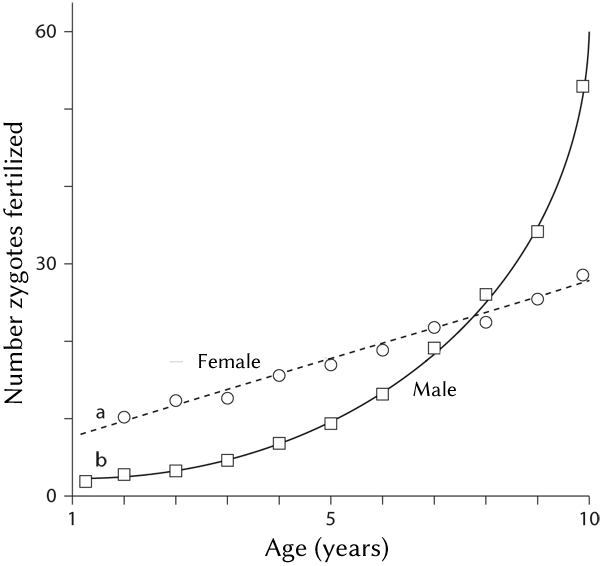
\includegraphics[width=0.45\textwidth]{seq_hermaph_protogyny}\\
	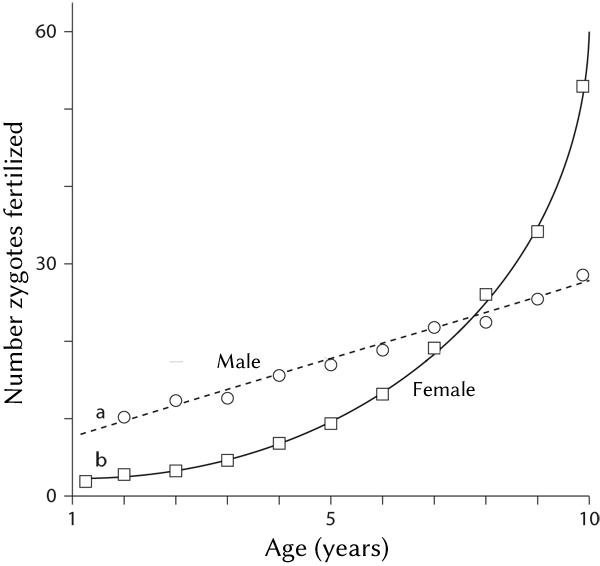
\includegraphics[width=0.45\textwidth]{seq_hermaph_protandry}\\
	
	\vspace*{-2\baselineskip}\hfill\tiny Modified from Avise and Mank 2009.

\end{multicols}

% Protandry answer
\AnswerBox{0.01\textheight}{Protandry (1 pt). Males have higher fitness than females at a younger age. Females have greater fitness at later age (2 pts). Being male first and female second increases fitness over the lifetime of the individual (2 pts)}
%

\newpage

%\begin{equation}\label{key}
\question
\begin{multicols}{2}
Male treehoppers (genus \textit{Enchenopa}) attract females by sending vibrations through plants. One species sends low frequency vibrations through the stem of a plant. The other species sends high frequency vibrations through the petiole.  The frequency differences of the males maximize detection by their respective females in the same environment (McNett and Cocroft 2008).

\columnbreak

	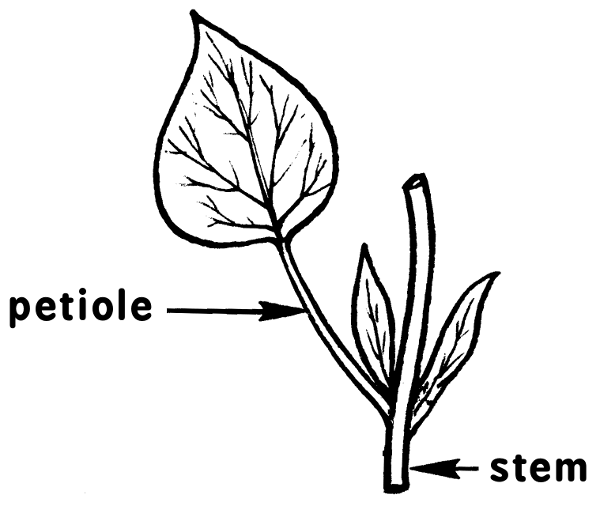
\includegraphics[height=1.75in]{petiole_stem}
\end{multicols}

	\begin{parts}
	\part[5]
	Is this intrasexual or intersexual selection? Why?
	
	\AnswerBox{0.1\textheight}{%
	Intersexual. Females are choosing males based on a characteristic of the male.
	}
	
	\part[10]
	Did the frequency differences more likely evolved by sensory bias or sensory drive? Explain what is sensory bias or sensory drive (depending on your choice), and then explain how your choice is consistent with the scenario described above.

	\AnswerBox{0.3\textheight}{%
	Sensory drive. Sensory drive is when female drives evolution of a trait based on the ability of the trait to stand out from the environment. Here, the different vibrations standout relative to their environments.
	}
	\end{parts}

%\end{equation}
\newpage

\question[10]
Persimmion trees produce either male flowers (no carpels) or female flowers (no stamens). Use the floral quartet model to explain which (if any) class or classes of MADS genes could be lost (no expression) to produce 1) male flowers and 2) female flowers. If the model does not work for one or both sexes of flowers, explain why for each sex.

\question[5]
On screen is a goosefish. It has an unusually wide jaw compared to most fishes. You wish to explore which toolkit genes might be involved. Based on your knowledge of previous studies, which toolkit gene or genes would you be most likely to start with? Briefly explain why.



\question[15]
Strasburg et al.~(2007) tested whether the disjunct distribution of an Australian gecko, \textit{Heteronotia binoei}, was due to vicariance or range expansion. The distribution is indicated by the black dots in the inset below.  Below is a simplified version of their parsimony network.  Based on the network, state which hypothesis is supported and describe how the network supports the hypothesis you chose. 

Each circle represents one allele. Shading corresponds to the population sampled; grey is the western cluster and white is the central cluster. Each line connecting two circles indicates one mutation difference between alleles.  Small dashes indicate additional mutational differences between alleles.

	{\centering
	\includegraphics[width=0.95\textwidth]{gecko_network_trimmed}\par}

	\AnswerBox{0.2\textheight}{
	The western (grey) clade shows considerable genetic diversity, suggesting it is older and was likely a refuge. The central (white) clade has little genetic diversity, suggesting it is much younger and therefore the result of recent range expansion.
	}


%\vfill

%\bonusquestion
Select whether you want \textbf{2 points} or \textbf{5 points} added to your score for this exam. Before you decide, there is a small catch: if more than 10\% of the class selects 5 points, then no one gets the extra points. Only I will see your choice.

\begin{oneparchoices}
	\choice 2 points.
	\choice 5 points.
\end{oneparchoices}
	
\end{questions}

\end{document}